\documentclass[11pt]{article}
\usepackage{worksheet_style}

%\worksheetfilledtrue
\begin{document}
\worksheetheader{19}{Line Integrals}

\begin{background}
With vector fields defined, we now integrate them along curves. The line integral $\int_C \vect{F}\cdot d\vect{r}$ computes the work done by a force along a path. For conservative fields, the Fundamental Theorem of Line Integrals gives us a shortcut: the integral depends only on the endpoints, not the path.
\end{background}

\wsection{Contour Types}

A \textbf{contour} (or \textbf{curve}) $C$ is a path in $\R^2$ or $\R^3$ given by a parameterization $\vect{r}(t)$, $a \le t \le b$.

\begin{defbox}{Types of Contours}
\begin{itemize}[nosep, leftmargin=*]
  \item \textbf{Open} -- endpoints $\vect{r}(a) \neq \vect{r}(b)$
  \item \textbf{Closed} -- $\vect{r}(a) = \vect{r}(b)$ (loop); use notation $\oint_C$
  \item \textbf{Simple} -- does not cross itself
  \item \textbf{Piecewise smooth} -- finitely many smooth pieces joined end-to-end
\end{itemize}
\end{defbox}

\begin{center}
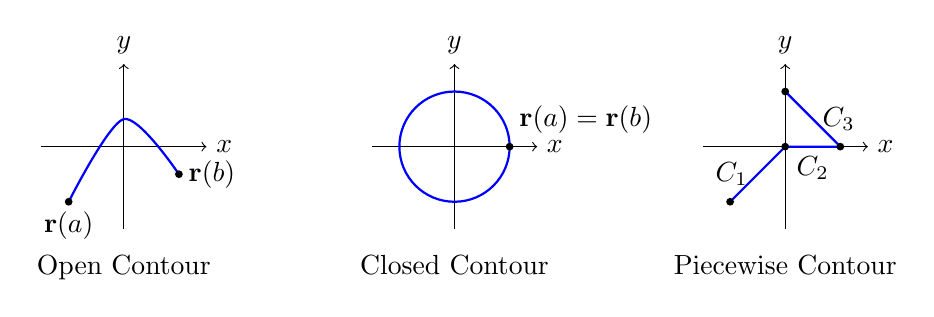
\begin{tikzpicture}[scale=0.7]
    % Open Contour
    \begin{scope}[xshift=-6cm]
        \draw[->] (-1.5,0) -- (1.5,0) node[right] {$x$};
        \draw[->] (0,-1.5) -- (0,1.5) node[above] {$y$};
        \draw[blue, thick] plot[smooth] coordinates {(-1,-1) (0,0.5) (1,-0.5)};
        \fill (-1,-1) circle (2pt) node[below] {$\mathbf{r}(a)$};
        \fill (1,-0.5) circle (2pt) node[right] {$\mathbf{r}(b)$};
        \node[below] at (0,-1.8) {Open Contour};
    \end{scope}

    % Closed Contour
    \begin{scope}[xshift=0cm]
        \draw[->] (-1.5,0) -- (1.5,0) node[right] {$x$};
        \draw[->] (0,-1.5) -- (0,1.5) node[above] {$y$};
        \draw[blue, thick] (1,0) arc (0:360:1);
        \fill (1,0) circle (2pt) node[right] {};
        \fill (1,0.5) circle (0pt) node[right] {$\mathbf{r}(a)=\mathbf{r}(b)$};
        \node[below] at (0,-1.8) {Closed Contour};
    \end{scope}

    % Piecewise Contour
    \begin{scope}[xshift=6cm]
        \draw[->] (-1.5,0) -- (1.5,0) node[right] {$x$};
        \draw[->] (0,-1.5) -- (0,1.5) node[above] {$y$};
        \draw[blue, thick] (-1,-1) -- (0,0) -- (1,0) -- (0,1);
        \fill (-1,-1) circle (2pt);
        \fill (0,0) circle (2pt);
        \fill (1,0) circle (2pt);
        \fill (0,1) circle (2pt);
        \node[left] at (-0.5,-0.5) {$C_1$};
        \node[below] at (0.5,0) {$C_2$};
        \node[right] at (0.5,0.5) {$C_3$};
        \node[below] at (0,-1.8) {Piecewise Contour};
    \end{scope}
\end{tikzpicture}
\end{center}

\wsubsection{Common Parameterizations}

\begin{itemize}[nosep, leftmargin=*]
  \item Line segment from $A$ to $B$ -- $\vect{r}(t) = (1-t)A + tB$, \; $t \in [0,1]$
  \item Circle $x^2+y^2 = R^2$ -- $\vect{r}(t) = \vec{R\cos t,\, R\sin t}$, \; $t \in [0,2\pi]$
  \item Graph $y = f(x)$, $a \le x \le b$ -- $\vect{r}(t) = \vec{t,\, f(t)}$, \; $t \in [a,b]$
  \item Helix -- $\vect{r}(t) = \vec{a\cos t,\, a\sin t,\, bt}$
\end{itemize}

\wsection{Scalar Line Integrals}

\begin{defbox}{Scalar Line Integral}
For a scalar function $f$ along a curve $C$ parameterized by $\vect{r}(t)$:
\[\int_C f\,ds = \wbml{\int_a^b f(\vect{r}(t))\,\|\vect{r}\,'(t)\|\,dt}\]
-- $ds = \|\vect{r}\,'(t)\|\,dt$ is the \textbf{arc length element}

-- \textbf{Interpretation:} area of the ``curtain'' under $f$ along $C$

-- Direction does not matter: $\int_C f\,ds = \int_{-C} f\,ds$
\end{defbox}

\begin{center}
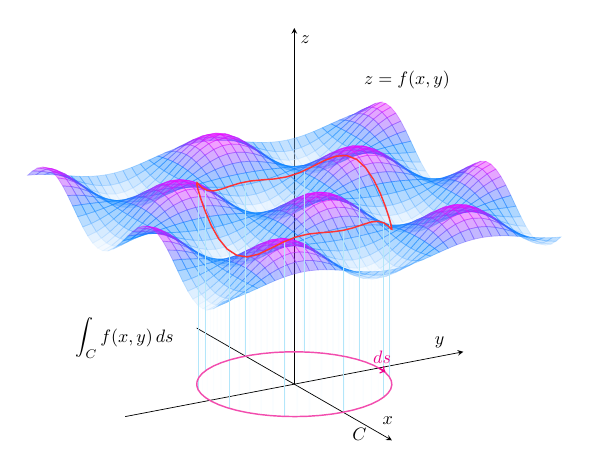
\begin{tikzpicture}[scale=0.65]
\begin{axis}[
    view={60}{20},  % Adjusted view angle for better visibility underneath
    axis lines=middle,
    xlabel={$x$},
    ylabel={$y$},
    zlabel={$z$},
    grid=none,
    ticks=none,
    width=12cm,
    height=12cm,
    xmin=-3, xmax=3,
    ymin=-3, ymax=3,
    zmin=0, zmax=4,  % Lifted up the z-range
    samples=40,
    domain=-3:3,
    y domain=-3:3,
    colormap/cool,
    clip=false
]

% Draw the undulating surface
\addplot3[
    surf,
    faceted color=blue!10,  % Made surface color lighter
    opacity=0.4,  % More transparent
    shader=flat,
] {2 + 0.3*sin(deg(2*x))*cos(deg(2*y))};  % Centered and lifted surface

% Fill the area under the curve with semi-transparent sheets
\pgfplotsinvokeforeach{0,0.02,...,1}{
    % Create fill between curve and xy-plane
    \addplot3[
        fill=cyan!20,  % Light cyan fill
        opacity=0.1,  % Very transparent for layered effect
        draw=none
    ] coordinates {
        ({1.5*cos(360*#1)}, {1.5*sin(360*#1)}, 0)
        ({1.5*cos(360*#1)}, {1.5*sin(360*#1)}, {2 + 0.3*sin(deg(3*cos(360*#1)))*cos(deg(3*sin(360*#1)))})
        ({1.5*cos(360*#1 + 1)}, {1.5*sin(360*#1 + 1)}, {2 + 0.3*sin(deg(3*cos(360*#1 + 1)))*cos(deg(3*sin(360*#1 + 1)))})
        ({1.5*cos(360*#1 + 1)}, {1.5*sin(360*#1 + 1)}, 0)
    };
}

% Draw vertical lines for the "curtain" effect
\pgfplotsinvokeforeach{0,0.1,...,1}{
    \addplot3[cyan!30, thin] coordinates {
        ({1.5*cos(360*#1)}, {1.5*sin(360*#1)}, 0)
        ({1.5*cos(360*#1)}, {1.5*sin(360*#1)}, {2 + 0.3*sin(deg(3*cos(360*#1)))*cos(deg(3*sin(360*#1)))})
    };
}

% Draw the curve on the surface
\addplot3[
    red!80,  % Slightly dimmer red
    thick,
    samples=50,
    domain=0:360,
] ({1.5*cos(x)}, {1.5*sin(x)}, {2 + 0.3*sin(deg(3*cos(x)))*cos(deg(3*sin(x)))});

% Draw the projected curve on xy-plane
\addplot3[
    magenta!70,  % Dimmer magenta
    thick,
    dashed,
    samples=50,
    domain=0:360,
] ({1.5*cos(x)}, {1.5*sin(x)}, 0);

% Add labels
\node[anchor=north] at (axis cs:2,0,0) {$C$};
\node[anchor=south] at (axis cs:0,2,3) {$z=f(x,y)$};
\node[anchor=west] at (axis cs:0,-4,1) {$\displaystyle\int_C f(x,y)\,ds$};

% Add a small ds element indicator
\draw[magenta,->,thick] (axis cs:0,1.5,0) -- (axis cs:0.2,1.5,0) node[midway,above] {$ds$};

\end{axis}
\end{tikzpicture}
\end{center}

\begin{example}[Scalar Line Integral Along a Line Segment]
Evaluate $\ds\int_C (x + 2y)\,ds$ where $C$ is the segment from $(0,0)$ to $(3,4)$.

\wbbox{
1. \textbf{Parameterize:} $\vect{r}(t) = \vec{3t,\, 4t}$, $t \in [0,1]$

2. \textbf{Speed:} $\vect{r}\,'(t) = \vec{3, 4}$, \; $\|\vect{r}\,'\| = \sqrt{9+16} = 5$

3. \textbf{Substitute:} $f(\vect{r}(t)) = 3t + 2(4t) = 11t$

4. \textbf{Integrate:} $\ds\int_0^1 11t \cdot 5\,dt = 55 \int_0^1 t\,dt = 55 \cdot \frac{1}{2} = \boxed{\dfrac{55}{2}}$
}{4.5cm}
\end{example}

\wsection{Vector Field Line Integrals}

\begin{defbox}{Line Integral of a Vector Field}
For a vector field $\vect{F}$ along a curve $C$:
\[\int_C \vect{F}\cdot d\vect{r} = \wbml{\int_a^b \vect{F}(\vect{r}(t))\cdot\vect{r}\,'(t)\,dt}\]
-- \textbf{Interpretation:} \wbi{work done by the force $\vect{F}$ along path $C$}{7cm}

-- Reversing direction \textbf{negates} the integral: $\int_{-C}\vect{F}\cdot d\vect{r} = -\int_C\vect{F}\cdot d\vect{r}$

-- Equivalent notation: $\int_C P\,dx + Q\,dy + R\,dz$
\end{defbox}

\begin{example}[Work Around a Circle]
Compute $\ds\int_C \vect{F}\cdot d\vect{r}$ for $\vect{F} = \vec{-y,\, x}$ along the circle $x^2+y^2=4$ (CCW).

\wbbox{
1. \textbf{Parameterize:} $\vect{r}(t) = \vec{2\cos t,\, 2\sin t}$, \; $\vect{r}\,' = \vec{-2\sin t,\, 2\cos t}$, \; $t \in [0,2\pi]$

2. \textbf{Evaluate $\vect{F}$:} $\vect{F}(\vect{r}(t)) = \vec{-2\sin t,\, 2\cos t}$

3. \textbf{Dot product:} $\vect{F}\cdot\vect{r}\,' = (-2\sin t)(-2\sin t) + (2\cos t)(2\cos t) = 4\sin^2 t + 4\cos^2 t = 4$

4. \textbf{Integrate:} $\ds\int_0^{2\pi} 4\,dt = \boxed{8\pi}$
}{5cm}
\end{example}

\wsection{Fundamental Theorem of Line Integrals (FTOLI)}

\begin{thmbox}{Fundamental Theorem of Line Integrals}
If $\vect{F} = \nabla f$ (conservative) and $C$ goes from $A$ to $B$:
\[\boxed{\int_C \nabla f \cdot d\vect{r} = f(B) - f(A)}\]

\textbf{Consequences:}
\begin{itemize}[nosep]
  \item The integral depends only on \wbi{the endpoints}{3cm} -- \textbf{path independence}
  \item For any closed curve: $\oint_C \nabla f \cdot d\vect{r} = \wbm{0}$
  \item If $\oint_C \vect{F}\cdot d\vect{r} \neq 0$ for some closed $C$, then $\vect{F}$ is \textbf{not} conservative
\end{itemize}
\end{thmbox}

\begin{example}[Applying FTOLI]
Evaluate $\ds\int_C \vec{ye^{xy},\, xe^{xy}}\cdot d\vect{r}$ from $(0,0)$ to $(1,2)$.

\wbbox{
1. \textbf{Recognize:} From Worksheet~21, $\vect{F} = \nabla f$ with $f(x,y) = e^{xy}$

2. \textbf{Apply FTOLI:} $\ds\int_C \vect{F}\cdot d\vect{r} = f(1,2) - f(0,0) = e^{(1)(2)} - e^{0} = \boxed{e^2 - 1}$

No parameterization needed --- any path from $(0,0)$ to $(1,2)$ gives the same answer.
}{3cm}
\end{example}

\begin{example}[Piecewise 3D Line Integral]
Evaluate $\ds\int_C \vect{F}\cdot d\vect{r}$ for $\vect{F} = \vec{y^2,\, z^2,\, x^2}$ along the path $(0,0,0) \to (1,0,0) \to (1,1,0) \to (1,1,1)$.

\wbbox{
\textbf{Segment 1:} $(0,0,0) \to (1,0,0)$: \; $\vect{r} = \vec{t,0,0}$, $\vect{r}\,' = \vec{1,0,0}$

$\vect{F} = \vec{0,0,t^2}$, \; $\vect{F}\cdot\vect{r}\,' = 0$. \; Integral $= 0$.

\textbf{Segment 2:} $(1,0,0) \to (1,1,0)$: \; $\vect{r} = \vec{1,t,0}$, $\vect{r}\,' = \vec{0,1,0}$

$\vect{F} = \vec{t^2,0,1}$, \; $\vect{F}\cdot\vect{r}\,' = 0$. \; Integral $= 0$.

\textbf{Segment 3:} $(1,1,0) \to (1,1,1)$: \; $\vect{r} = \vec{1,1,t}$, $\vect{r}\,' = \vec{0,0,1}$

$\vect{F} = \vec{1,t^2,1}$, \; $\vect{F}\cdot\vect{r}\,' = 1$. \; Integral $= \int_0^1 1\,dt = 1$.

\textbf{Total:} $0 + 0 + 1 = \boxed{1}$
}{7cm}
\end{example}

\begin{practice}

\prob
Evaluate $\ds\int_C xy\,ds$ where $C$ is the line segment from $(0,0)$ to $(1,1)$.

\wans{$\wbm{\dfrac{\sqrt{2}}{3}}$}

\vspace{3cm}

\prob
Evaluate $\ds\int_C \vec{y^2,\, 2xy}\cdot d\vect{r}$ from $(0,0)$ to $(1,1)$ along $y = x^2$.

\wans{$\wbm{1}$}

\vspace{3.5cm}

\prob
Evaluate $\ds\oint_C \vec{x^2,\, y^2}\cdot d\vect{r}$ where $C$ is the unit circle. (\textit{Hint: is the field conservative?})

\wans{$\wbm{0}$}

\vspace{2.5cm}

\prob
Evaluate $\ds\int_C \vec{2xz + y,\; x + z^2,\; x^2 + 2yz}\cdot d\vect{r}$ from $(0,0,0)$ to $(1,2,3)$ using FTOLI.

(\textit{Hint: find the potential function first.})

\wans{$\wbml{f = x^2z + xy + yz^2;\quad f(1,2,3) - f(0,0,0) = 3+2+18 = 23}$}

\vspace{4cm}

\prob
Evaluate $\ds\int_C (x^2 + y^2)\,ds$ where $C$ is the helix $\vect{r}(t) = \vec{\cos t,\, \sin t,\, t}$, $0 \le t \le 2\pi$.

\wans{$\wbm{2\sqrt{2}\,\pi}$}

\vspace{3cm}

\end{practice}

\end{document}
